\documentclass[10pt]{article}

\addtolength{\textwidth}{1in}    
\addtolength{\hoffset}{-0.5in}
\addtolength{\textheight}{1.5in}
\addtolength{\voffset}{-1in}

\setlength{\parskip}{\baselineskip}
\addtolength{\topsep}{-\baselineskip}
\setlength{\parindent}{0em}
\renewcommand{\familydefault}{\sfdefault}

\usepackage{../Utils}
\usepackage{eurosym}


\bc

    * Introduction --short description of the project and goals;
    * Description of innovation:
          o the problem solved by this project;
          o the relative advantage of the proposed innovation;
          o usability: for whom and to what purpose;
          o perspectives for further development of this innovation and/or other technologies. 
    * Project setup --organizational, technical, eventual partners, dependencies on other projects, licenses, and such;
    * Project planning --milestones and related results;
    * Project budgeting;
    * Project risks --which risks can be overseen from the start of the project;
    * Project results dissemination --how the project team is going to disseminate results and to whom, publicity, diffusion of the produced innovation;
    * Possibly, follow-ups on the project. 

\ec


\title{Proxima 2.0: WYSIWYG generic editing for Web 2.0\\
\bigskip
        \large NLnet project plan}
\author{dr Martijn M. Schrage\\
        \small Dept. of Computing Sciences, Utrecht University\\
        \small {\tt martijn@cs.uu.nl}
        }
\date{}
\begin{document}

\maketitle


\head{Abstract}\\
In line with the Web 2.0 trend, an increasing number of web sites offer visitors the possibility to modify and add content through some form of editing. However, the editors provided are either basic text editors that are awkward for editing complex presentations, or custom-made editors for a specific type of content. A generic editor could be used to create powerful editors with little effort, but has the problem that it needs to be installed on each machine it is used on.

A server-based generic editor can solve this problem. It will allow the easy creation of WYSIWYG editors on web-pages, without requiring the editing user to install any software. Instead, the browser runs a simple script that draws a rendering of the edited content and sends edit events back to the server.

The Proxima generic editor system has a layered architecture that can be modified in a straightforward way to support a client-server model. Because of the powerful presentation language of Proxima, web-based WYSIWYG editors for a wide range of document types can be created with little effort. The edited documents are stored as XML.

\head{What the NLnet contributions will be used for}\\
The NLnet contribution will be used to realize the web-based client-server version of Proxima. Furthermore, a number of interesting editors will be instantiated to showcase the capabilities of the system, thus helping to  attract the attention of possible contributors to the project.


\head{Comparison with other projects}\\
The project can be compared with two kinds of existing projects: web-based editors and generic editors.

A multitude of web-based editors exist. Examples are Wiki's, the Yahoo!\ Pipes editor, and Google Docs suite. However, these editors are either mainly textual or WYSIWYG but targeted at a single type of document. No existing project offers generic web-based editing.

There are not many generic editing projects that are still being maintained. One example is Citrus (http://www.cs.cmu.edu/~NatProg/citrus.html). On the other hand, also XML editors can be regarded as generic editors, but the existing XML editors that are powerful enough to create interesting WYSIWYG editors, such as XMetaL and XMLSpy, have no support for creating web-based versions of these editors, and neither does Citrus.

The Proxima 2.0 project will be unique in the sense that it will combine WYSIWYG generic editing with web-based editing.

\section{Introduction}
%    * Introduction --short description of the project and goals;

\subsection{Project description}

% web 2.0 more editors. Editors are basic. Complex editors tricky. hand-held devices.
With the advance of Web 2.0, an increasing number of web sites offer visitors the possibility to create content by editing the content of the visited page. An example is Wikipedia, which allows anyone visiting the site to edit its content.

Ideally, a visitor should be able to modify and add content in a WYSIWYG fashion:  during editing, the content looks the same way as when only viewing it. But unfortunately this is often not the case. For example, in Wikipedia, the editor offers a plain text view of the edited content. Hence, text markup such as bold and italic styles are shown as tags in the editor. Moreover, a graphical entity such as a mathematical formula is shown as text as well. For example, during editing, the simple formula $b^2 = a^2 + ab$ is shown as:
 
\begin{center}
\verb|''b''<sup>2</sup>&nbsp;=&nbsp;''a''<sup>2</sup>&nbsp;+&nbsp;''ab''|
\end{center}

Buttons are available for inserting the text for certain tags, but these work purely textual. Hence it is possible to insert a new tag in the text of another tag (e.g.\ \verb|<s<sup>up>|), thereby invalidating the structure. Furthermore, when an invalid structure arises, the editor offers no support to fix it or point out where the problem is. 

Some sites provide more advanced editors that exhibit WYSIWYG behavior. An example of this is the editor for Yahoo!\ Pipes\footnote{Yahoo!\ Pipes: \url|http://pipes.yahoo.com|}, which provides a graphical interface for creating web-based applications using web services from various sources (so-called mash-ups). Structures can be created by dragging components onto a canvas, editing their properties, and connecting their input and output ports. Though powerful, such custom-made editors require a significant engineering effort, which puts them out of reach for many applications.

Another problem with custom-made editors is that it is difficult to combine them. If a Wiki site makes use of plug-ins, each coming with its own specific editor, it is not always possible to combine the plug-in editors into a single editor. Instead, a page will be a collection of editors, each with its own specific edit model, undo buffer, etc.

The problem of building  editors can be tackled by using a generic editing framework. When provided with the type of the edited content together with a description of its presentation and the edit behavior, a generic editor functions as an editor for that specific type of document. However, this solution would require the installation of this generic editor on each device that is used to edit content.


\bc
Furthermore, a complex editor requires a considerable amount of processing power from the device on which the page is edited. This is not an issue for a desktop or laptop computer, but web pages are being viewed increasingly on small handheld devices and mobile phones. 
\todo{noemen?}
\ec


Because Internet connections nowadays are fast and widely available, a better solution to this problem is to use a web-based generic editor. The editor runs on a server and communicates with a light-weight Ajax client that runs in a browser and draws a rendering of the edited content while sending back edit events. 

The Proxima editor\footnote{Proxima homepage: \url|http://www.cs.uu.nl/research/projects/proxima|} is a generic editor with an architecture that is very well suited to support such a client-server model of editing. The resulting web-based editor can provide WYSIWYG editing functionality for web pages with only a fraction of the effort required to build a custom-made editor. Proxima is an open-ended system: new object types and presentations can be added to enable the creation of increasingly powerful document types. Moreover, editors for different kinds of content can easily be combined. Hence, we can provide edit functionality similar to a textual Wiki, but with a much richer underlying document type. Text can have visual markup, such as different fonts and colors, and editable graphical entities such as formulas can be combined with the textual content. The edited content can be stored as XML. The client consists of a light-weight Ajax script, so no plug-in needs to be installed. Lastly, the editors will have little processing impact on the device that is used to edit the page. 

%\todo{mention pipes and more editors here? (and mention we can't do pipes yet?)}

The migration from desktop applications to server-based applications is already taking place in other areas. E-mail clients are a good example. The first web interfaces were rather static, but more recent Ajax interfaces such as GMail and Yahoo!\ allow access to e-mail and folders comparable to stand-alone mail clients. Although a mail client requires less communication than an editor, applications of Virtual Network Computing show that server-based applications that let all processing be done by the server are feasible. Moreover, since a generic editor need not simply send a bitmap but can send a much more efficient incremental update, the experienced responsiveness will be much higher than with an editor running over a VNC-based protocol.

\subsection{Project goals}

The primary goal of this project is to create the web-based client-server version of Proxima, for which a proof-of-concept implementation has already been constructed. This consists of modifying the rendering part of Proxima to act as a server and communicate with an external rendering client. The client itself will be a light-weight Ajax script that draws the rendering of the document and captures edit events. The client will run in any major browser on any major platform, without the need to install any plug-ins.  

A secondary goal is to showcase the potential of the Proxima technology in order to attract the attention of possible contributors. The hope is that eventually a vibrant community will contribute to a shared repository of resources and push the development of Proxima beyond what a small academia-based group can hope to achieve by itself. 
%\todo{mention that implemented web-page editors will provide good showcase?}


\bc

Using Ajax and Flash technology, user-friendly WYSIWYG editors can be created. Take for example the editor for Yahoo!\ Pipes~\cite{yahoo08pipes}, which provides a graphical interface to create web-based applications using web services from various sources. However, such editors are hard to build. Furthermore, a complex editor requires a considerable amount of processing power from the device on which the page is edited. This is not an issue for a desktop or laptop computer, but web pages are being viewed increasingly on small handheld devices and mobile phones. 

% internet getting better. Create server-based editor
At the same time, the availability of (wireless) Internet is on the rise, with connection speeds rising and costs dropping. Hence, it makes sense to take the editor application away from the local device, and create a server-based editor that processes edit events and communicates changes in the presentation to a light-weight client. The fact that this is feasible can be seen from technologies such as Virtual Network Computing (VNC).

% Proxima good for making editors
The Proxima generic editor~\cite{schrage08proximaHome, schrage04proxima} can be used to easily create WYSIWYG editors for a wide range of document types. An editor can be instantiated by specifying a document type, a document presentation and the edit behavior. Presentations can be a mix of text and graphical elements.The resulting editors allow edit operations on the document structure as well as on its screen representation (i.e.\ free-text editing), without the need to switch between the two modes.

% easy to maked server-based
Because of its architecture, it is straightforward to provide Proxima with a web-based interface. Instead of rendering the presentation to a screen, the updates on the rendering are sent over an HTTP connection to a remote client. The client has a light-weight Ajax renderer that draws the rendering on the browser screen and captures mouse and keyboard events, which are sent back. Since the Proxima has support for incrementality, only updates to the rendering are sent to the client.

\ec

% Project goal


\section{Project description}
%    * Description of innovation:
%          o the problem solved by this project;
%          o the relative advantage of the proposed innovation;
%          o usability: for whom and to what purpose;

\subsection{The problem} 

%web 2.0 meer editing, basic
Web 2.0 sites, such as wiki sites (e.g.\ Wikipedia), social network sites (e.g.\ Myspace), or auction sites (e.g.\ eBay) allow visitors to add or modify the content on the page. The facilities for editing, however, are often rather basic. 

% beter kan, maar is duur.
It is possible to provide custom-made WYSIWYG editors, for example, by using Javascript or Flash, or through plug-ins. Examples are the advanced graphical editor for Yahoo!\ pipes, and the editors that are part of Google docs suite. Regarding functionality, these systems approach desktop applications. However, the effort required to build such a custom editor is considerable.

It would be desirable to be able to quickly build advanced WYSIWYG editors for specific content that can be included on any web page, without the need to install any plug-ins on the cient machine.


\bc
% internet sneller apparaten kleiner.
% take editor application away from the client.
Another trend is that the availability and speed of Internet connections is increasing, while the costs are dropping. A logical step therefore is to state of affairs suggests that the time is ripe for web-based editors. Rather than running a local editor application, the local machine only runs a light-weight client, which is also suitable for devices with little processing power. A server computes a rendering of the document, which is sent to the local client. The client draws the rendering on the screen and catches mouse and keyboard events, which are sent back to the server. Subsequently, the server computes the corresponding update on the rendering and sends it to the client.

% in e-mail we see it already
The migration from desktop applications to server-based applications is already taking place in other areas. E-mail clients are a good example. The first web interfaces were rather static, but more recent Ajax interfaces such as GMail and Yahoo!\ allow access to e-mail and folders comparable to stand-alone mail clients. Although a mail client requires less communication than an editor, applications of Virtual Network Computing show that server-based applications that let all processing be done by the server are feasible. Moreover, since a generic editor does not simply send a bitmap but a much more efficient incremental update, the speed will be much higher than when a VNC protocol is used for editing. 
\ec

\subsection{Proxima 1.0}
%Proxima. What is proxima and generic editing

Proxima is a generic editor system developed at Utrecht University. A generic editor is a system that can be used to create editors. In order to create, or {\em instantiate}, an editor, Proxima is specialized with a document type and a number of sheets describing the presentation of the document and its edit behavior. The content of a Proxima document can be mixed text, images and diagrams. A key feature of Proxima is that the instantiated editors are presentation-oriented, meaning that the user performs the edit operations on the fully formatted (WYSIWYG) presentation of the document. At the same time, edit operations on the document structure (such as changing a section to a subsection) are also possible. The document can be stored as XML or converted to another textual format. The system is written in the functional language Haskell and consists of about 15000 lines of code.

An example of an editor for a sophisticated document type created this way is the Dazzle documentation editor, an editor for the documentation of Bayesian networks. This editor combines graph editing with word-processor functionality. A document contains a Bayesian network (which is essentially a graph) and a list of sections, which contain a view on small part of the graph together with the documentation of that part. 

Figure~\ref{fig:bayesDocEditor} shows a screenshot of the editor. The graph in the figure is an editable subgraph of the main network, so any changes to the edges are also applied to the main network, thereby solving the major problem of maintaining consistency. In the text, tags can be added to denote a reference to a network node. The text also contains references to sections and figures, the numbers of which are automatically computed. Missing references are signaled with squiggly lines.

\begin{figure}[t]
\begin{center}
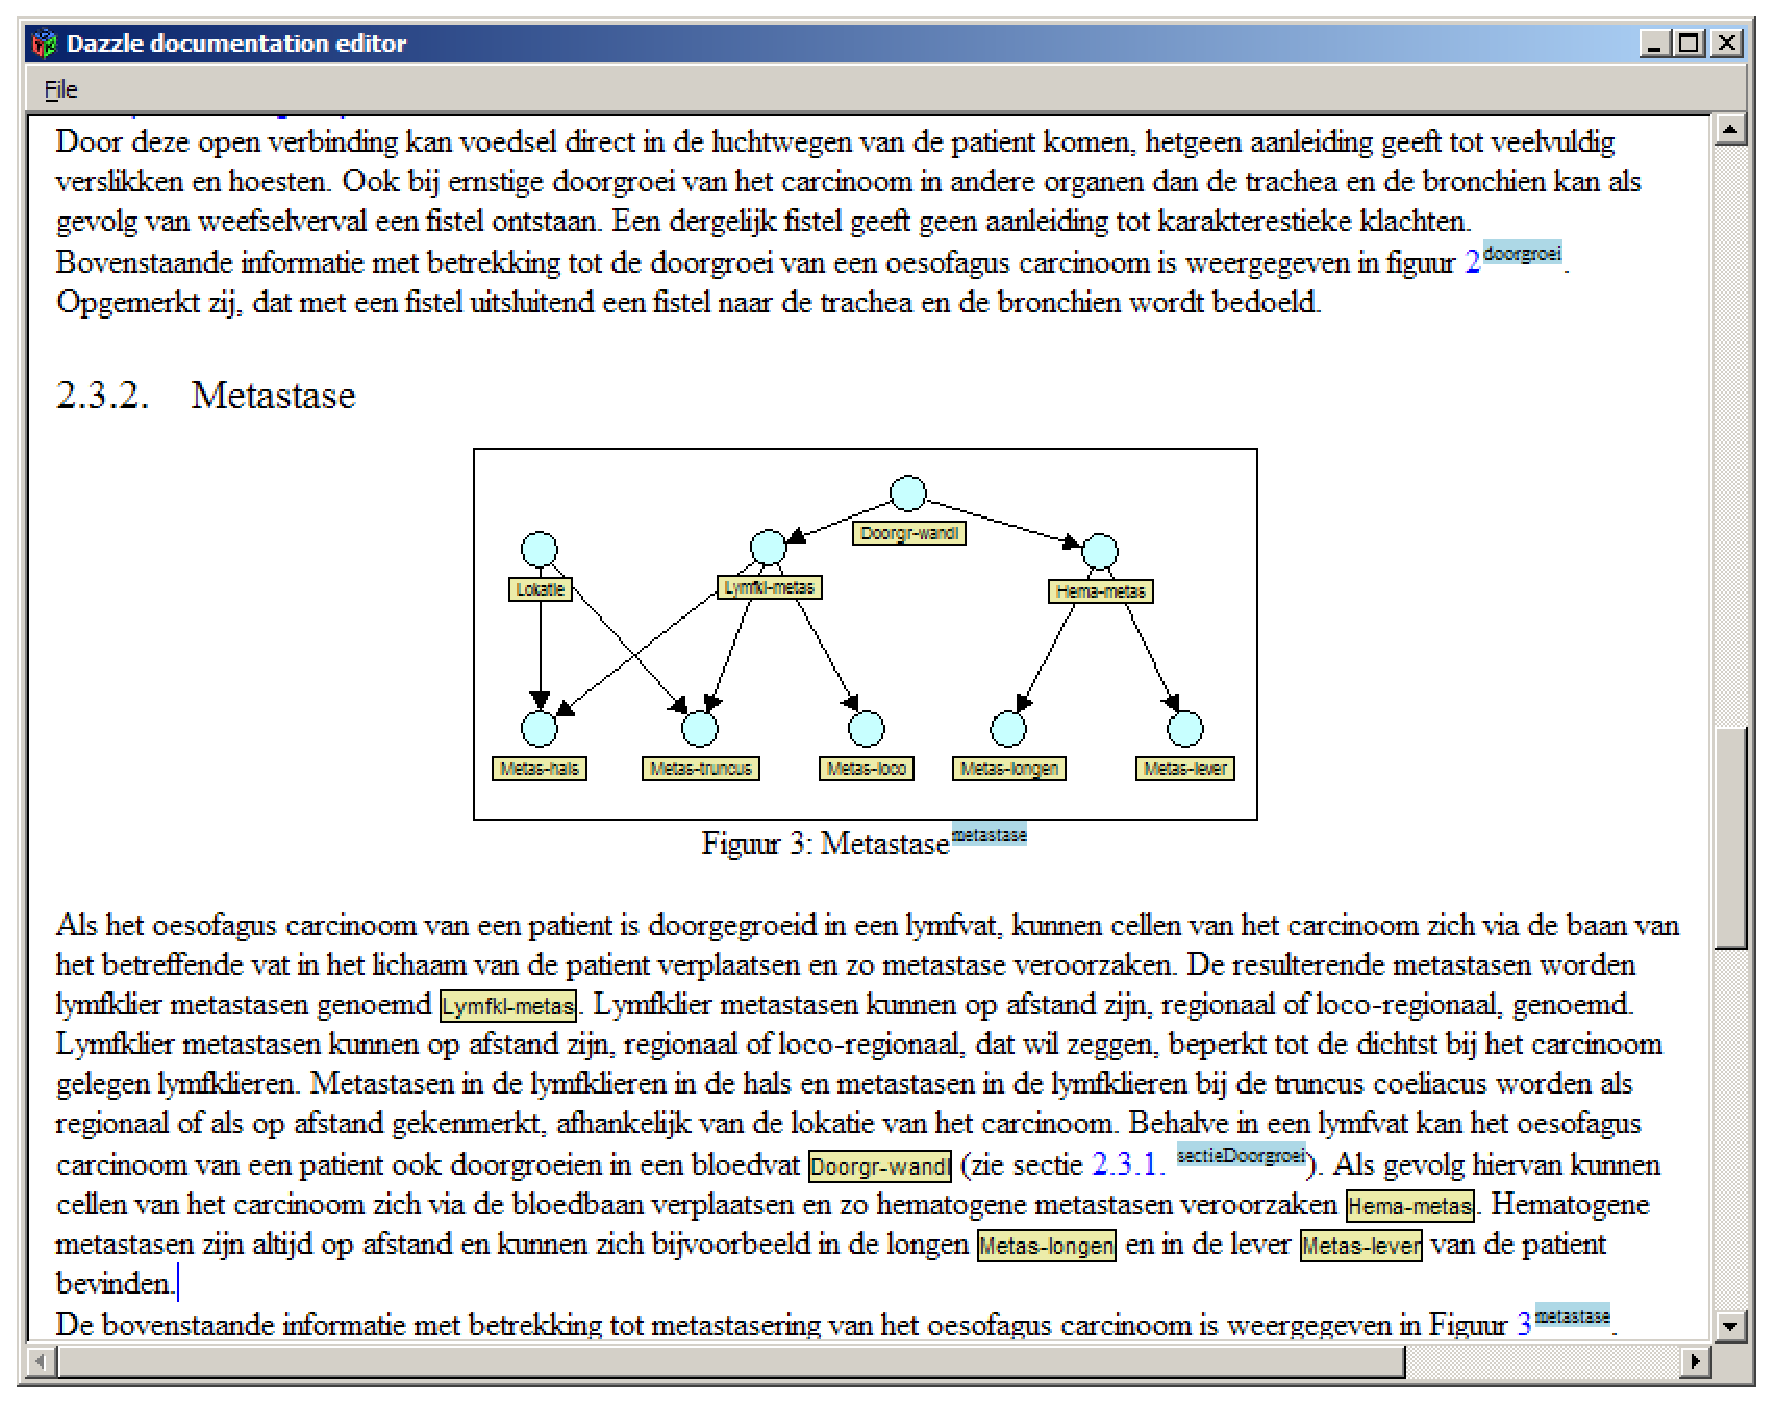
\includegraphics[width=12cm]{images/subgraph}
\end{center}
\caption{The Bayesian network documentation editor.}
\label{fig:bayesDocEditor}
\end{figure}

Another example of an editor that has been obtained from generic Proxima by instantiation is a source code editor for the functional language Helium (see Figure~\ref{fig:heliumEditor}). The editor shows parse and type errors in place, and allows for graphical presentations of language constructs. Structural edit operations can be combined with free-text editing. Hence, we can use structural edit operations to delete and insert list elements, which automatically removes and adds the necessary commas (or other separators). But at the same time, it is possible to delete the substring ``\p{+2, }'' from the expression ``\p{[ 1+2, 3]}'' (which does not correspond to a structural edit operation), resulting in ``\p{[ 13 ]}''.


An important aspect of Proxima is the fact that a presentation may contain computed values and structures. This is apparent in Figure~\ref{fig:heliumEditor} on the line before the declaration of \p{c}. The value \p{16} is computed automatically, and changes when parameter \p{3} is edited or when the function \p{f} is modified.

\begin{figure}
\begin{center}
\includegraphics[width=12cm]{images/heliumMainWindow}
\end{center}
\caption{The Helium editor.}
\label{fig:heliumEditor}
\end{figure}

Besides these two editors a multitude of editors can be implemented with Proxima. One can think of equation editors, spreadsheets, or text editors for the compact syntax of XML standards such as XML Schema\footnote{Compact syntax for XML Schema: \url|http://www.xml.com/pub/a/2003/08/27/xscs.html|} and Relax NG\footnote{Compact syntax for Relax NG: \url|http://www.xml.com/pub/a/2002/06/19/rng-compact.html|}, but also more exotic applications, such as a chess board, a family-tree editor, or an on-line multiple choice quiz that keeps track of the score.


\subsection{The Proxima architecture}

The core architecture of Proxima consists of a number of layers, each communicating with its upper and lower neighbors. The layered structure is based on the staged nature of the {\em presentation} process and its inverse, the {\em interpretation} process. The positions at which the document, the rendering, and the intermediate data structures reside are called {\em levels}. Between each pair of levels we have a {\em layer} that maintains the mappings between its adjacent levels. Each layer consists of a presentation component and an interpretation component and may be parameterized by a {\em sheet}. Figure~\ref{fig:levelsAndLayers} schematically shows the levels and layers of Proxima. From a document type definition, a code generator generates a number of Haskell modules, which are compiled together with the sheets and the Proxima base modules to yield an editor. 

\begin{figure}
\begin{center}
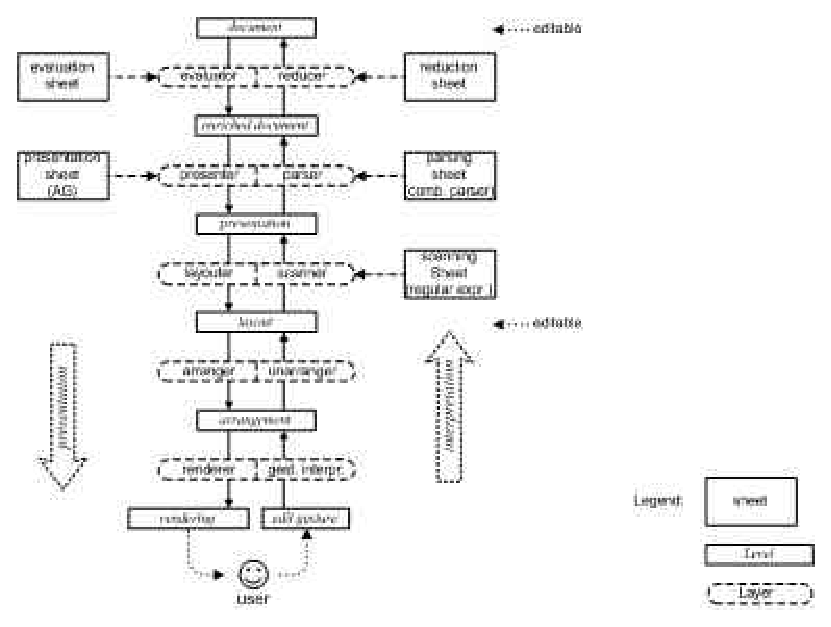
\includegraphics[width=12cm]{images/LayerOverview}
\end{center}
\caption{The levels and Layers of Proxima.}
\label{fig:levelsAndLayers}
\end{figure}

A data level in Proxima is not simply an intermediate value in the presentation computation. It is an entity in its own right and maintains part of the state of the editor. The six levels of Proxima are:


\bl
\o {\bf Document:} The document structure.

\o {\bf Enriched Document:} The document attributed with derived values and structures, such as the type of a function or a table of contents.

\o{\bf Presentation:} A logical description of the presentation of the document, consisting of rows and columns of presentation elements with attributes. The presentation also supports formatting based on available space (e.g.\ line breaking).

\o{\bf Layout:} A presentation with explicit white space. 
%, which does not contain tokens.

\o{\bf Arrangement:} A formatted layout with absolute size and position information.

\o{\bf Rendering:} A bitmap of the arrangement.
\el


\bc
We briefly discuss each of the five layers.

\head{Evaluation layer}\\
The evaluation layer takes care of computing derived structures and values over the document, and of mapping updates on these derived structures back to document updates. In this layer, for example, type inference may take place. The layer is parameterized by an {\em evaluation sheet} and a {\em reduction sheet}, which specify the mappings. 

\head{Presentation layer}\\
The presentation layer consists of the presenter and the parser. The presenter takes an enriched document tree and computes a presentation for it according to the {\em presentation sheet}. Its counterpart, the parser, maps a presentation tree back to an enriched document and is parameterized by a {\em parsing sheet}.

\head{Layout layer}\\
The layout layer handles automatic white space, which is maintained in the white-space map that is part of the presentation level. For each token, the layout component looks up the corresponding white space and inserts actual line breaks and spaces in the presentation. The scanner recognizes tokens in the layout level, based on regular expressions specified in the {\em scanning sheet}. It also stores white space in the white-space map. Because mapping tokens to strings is straightforward, the layout component does not need a sheet parameter.

\head{Arrangement layer}\\
In the presentation direction, the arrangement layer computes the precise position and size for each element in the layout level. It also handles line breaking. The arrangement level is not directly editable, so it need not be mapped back onto the layout level. Hence, the only thing that needs to be done in the interpretation direction, is to map absolute coordinates in edit commands to paths in the presentation tree. 

\head{Rendering layer}\\
The renderer creates a bitmap for the arrangement. In the other direction is the gesture interpreter, which maps edit gestures onto edit operations designated for the higher layers.

\ec

%\bl
%\o sometimes awkward, because we have to conform to the layers.
%\o but this has advantages: new GUI lib in a matter of days.
%\el



\bc
Presentation-oriented editing actually takes place at the layout level rather than the presentation level, thus allowing free-text editing also on white space (which is absent on the presentation level). Hence the two levels that are directly editable are the document level and the layout level. 
\ec

After an edit operation on the document, all levels from document to rendering are updated to reflect the update. After an edit operation on the layout level, the modified layout is scanned, parsed and reduced, to obtain the corresponding updated document, from which an updated rendering is computed. Scanning and parsing does not occur after every presentation edit operation. Depending on the editor, it may occur either on a navigation operation, after a certain time interval, or at an explicit request by the user.

In order to instantiate an editor, a number of so called {\em sheets} must be provided:

\bl
\o{\bf Document type definition:} 
A EBNF grammar representation of the document type. It is similar to a monomorphic Haskell data type or an XML Schema, with support for lists.

\o{\bf Presentation sheet:} 
An attribute grammar that specifies for each language construct how it is presented. Simple computations, such as section counters, or static checks on the document (e.g.\ whether a reference is defined) can be implemented as well.

\o{\bf Scanning sheet:}
A set of regular expressions for the tokens in the textual parts of the presentation.

\o{\bf Parsing sheet:} 
A module that contains the parsers for each part of the presentation that is presented textually.
\el

For most editors, the computations can be specified in the presentation sheet. However, for more complex editors, two extra sheets can be provided to deal with derived structures and values: the {\em evaluation sheet} and its inverse, the {\em reduction sheet}.  

\bl
\o{\bf Evaluation sheet:}
Can be used to specify derived structures, such as a table of contents, or a table with a structure that depends on information in the document. 

\o{\bf Reduction sheet:}

The reduction sheet specifies how updates on derived structures are mapped back onto the document. In many cases, derived values are not editable, in which case the reduction sheet simply ignores the value. However, in some cases, updates on a derived structure correspond to logical updates on the document. One can think of editing the title in a table of contents, or swapping two section titles, which causes the actual sections to swap as well. 
\el


\subsection{Proxima 2.0}

Turning Proxima into a web-based editor will have little impact on the overall implementation. Because of the strict separation between layers, enforced by the architecture, only four relatively small modules contain GUI-specific code. When the system needed to be ported to a new GUI library, this only took a couple of days. Hence, implementing support for an external renderer will be a relatively straightforward operation. In fact, an early version of Proxima actually used a stand-alone renderer client that it communicated with through a socket connection.

In order to realize the web-based functionality, three components need to be developed:

\bl
\o An HTTP server that sends a rendering to a client and retrieves the edit commands. 

\o A Proxima rendering module that renders the arrangement to an XML string that is handled by the client.

\o An Ajax client that renders a presentation on the screen and captures edit events, which are sent to the server.
\el

\subsubsection{The HTTP server}

A simple HTTP server will handle incoming requests and start a Proxima session for each new request. The Proxima session is quite similar to an ordinary Proxima session, except that instead of catching edit events directly and drawing the rendering updates on the screen, the events are received from a socket connection, and updates are sent over  this socket. This functionality can be added to the current GUI module, which contains the event loop that handles events and draws the rendering onto the screen. 
 
\subsubsection{The web-based renderer}

The current renderer creates drawing commands for the GTK windowing toolkit. It traverses the arrangement data structure, and produces commands for changed parts of the arrangement that are currently in view. The new renderer will be very similar but instead of computing a list of commands, it will produce an XML string.

\subsubsection{The Ajax client}

The main implementation effort of the project will be the Ajax client. It will capture mouse and keyboard events and send these to the Proxima server. In response, it will receive an XML structure corresponding to the update on the rendering. Textual parts of the rendering, as well as images, can be mapped onto DHTML elements. Other graphical elements, such as lines and circles, can be mapped onto SVG elements or drawn separately. The client will also show context menus and tooltips received from the server.

\bc
\subsection{Usability}

The usability of a web-based editor depends largely on its efficiency. The Proxima renderer only generates a rendering for that part of the presentation that is currently visible on the screen. Furthermore, because Proxima has support for incrementality, only updates to the rendering are sent over the socket, rather than the entire screen. Hence, most edit operations only causes a minimal amount of communication. Only when an update has a more global effect, the amount of data transferred will increase. Nevertheless, a small delay that occurs only once in a while is not a serious hindrance during editing. 

bc
At the moment, moved blocks are not recognized, since the screen renderer performed well enough without this. For web-based editors, however, this is more important, as the creation of a new line would cause half the page to be transmitted. Fortunately, the renderer provides hooks to be extended to recognize moved blocks, and create a move command for these.
ec

Another aspect of the usability is the latency in the server connection. Even if the transfer speed is high enough, there might be a delay in the response from the server. bc 
In order to handle this, the render can create a predictive rendering in response to an edit event, which is updated when the result of the server is received.
ec
A simple solution to this is to insert typed characters at the location of the focus in the current rendering, copying the style from surrounding characters, until the rendering update is received. Latency could also affect drag and drop editing, but a simple solution here is to show an outline of the focused object at the current mouse position. 

However, experiments with a simple web-based text editor have shown response times to be more than adequate over a wireless ADSL connection, even when several kilobytes of date wer transmitted. Hence, efficiency and latency are not expected to pose serious problems. 
\ec

\subsection{Relative advantage of proposed innovation}

The advantage of Proxima 2.0 is that it will make it easy to build advanced WYSIWYG editors for specific content. At the same time, these editors will not require any plug-ins installed on the client machine. Furthermore, Proxima editor servers can be easily hosted on any server.


\subsection{Usability}

One must distinguish between two levels of users of the web-based Proxima technology. One level are the people who generate specific Proxima instantiations by supplying the required sheets (in particular document type definition and presentation sheet). Except for very simple instantiations, creating these wholly anew requires considerable skills. However, as the repository of sheets grows, it will become increasingly possible to cobble new instantiations together by combining pre-existing elements.  Dedicated sheet editors (themselves instantiations of Proxima) can be created to assist in this task. In any case, even with the very limited current repository, generating an instantiation is definitely much less effort than creating an equivalent editor de novo.

The other level of users consists of the visitors of websites who use a site-specific instantiation of Proxima to edit content on web pages. Here the usability will depend on the specifics of the instantiation and the complexity of the application. Proxima offers powerful support for the editing tasks, as explained above.

% (Of course, there is no guarantee that an instantiation will actually make use of these.)


\subsection{Further development}
%          o perspectives for further development of this innovation and/or other technologies. 


When the web-based functionality has been added to Proxima, an obvious extension will be the connection of Proxima to a database. Documents are now internal data structures, but it will be interesting to obtain values or even subtrees of the document from a database. With this functionality, Proxima can be used as a front-end for web-based database applications.

A second area of further development is the underlying edit model of Proxima. Currently, presentation-oriented editing is supported on graphs and on textual presentations. The graph presentation can be extended to provide a more general framework in which objects can be positioned and connected at certain points. With such a generalization, it will become possible to implement editors similar to the Yahoo!\ Pipes editor.

Finally, as documents will get larger, the load on the server will increase. Proxima has several hooks for implementing incremental behavior: meaning that a change in the presentation only causes a small change in the document. Incrementality is already supported on the rendering level. Support for incrementality on other levels will mean that larger or more documents can be edited simultaneously.


\section{Project setup}
%    * Project setup --organizational, technical, eventual partners, dependencies on other projects, licenses, and such;

The work will be performed at the Software technology group of Utrecht University, lead by Prof.\,Dr.~S.\,D.~Swierstra. It will build upon the Proxima research project that was conducted by this group. The software technology has valuable expertise on the language Haskell, as well as on the technologies used in Proxima. Moreover, there is experties on Javascript and Ajax technology. The group will facilitate a laptop on which development can take place, and provide a server machine to host Proxima servers.

\bc
The group has expertise in many of the fields that are relevant for
this project.
Jeuring has developed several incremental algorithms, and has 
contributed significantly to the field of generic programming, amongst
others by developing XML tools. He is the principal investigator of
the Generic Haskell project (NWO, 2000-2004, \url{http://www.generic-haskell.org}),
the goal of which is to develop a language that supports the construction of generic
programs. Meertens has been at the forefront of the development of
theories for program calculation, and was one of the main
investigators of the Views project (CWI, Amsterdam, 1988--1994, 
\url{http://www.cwi.nl/~steven/views/}), 
and the Acela project (STW, 1993--1997, 
\url{http://www.cwi.nl/~steven/acela/}). An important subgoal of
these projects was to support the construction of interactive systems.

Finally, Swierstra has led the LRC project (UU, 1990--2000, 
\url{http://www.cs.uu.nl/groups/ST/Software/LRC/}). LRC is a system for generating 
efficient incremental attribute evaluators, and is used to generate 
language based editors and other advanced interactive environments.
\ec

The main implementation effort will be conducted by the requestor, Martijn Schrage, who has designed and implemented the Proxima system. He has over 10 years of experience writing large and complex software systems in Haskell. Before starting his PhD research on Proxima, he worked on a Java project for two years. After his PhD, he continued to work on Proxima and has also worked on the Haskell project Dazzle\footnote{Dazzle: \url|http://www.cs.uu.nl/dazzle/|}. Besides Haskell and Java, he is also proficient in the languages C\# and Javascript.

Other people involved with the project are Lambert Meertens and Doaitse Swierstra. Lambert Meertens was one of the main researchers on the Views\footnote{Views: \url|http://www.cwi.nl/~steven/views/|} and Acela\footnote{Acela: \url|http://www.cwi.nl/~steven/acela/|} projects, and has an extensive knowledge of presentation-oriented editing systems. Doaitse Swierstra has designed the parser library and attribute grammar system that form an integral part of the Proxima system. He has also worked on incremental attribute grammar evaluation and was one of the designers of the LRC system\footnote{LRC: \url|http://www.di.uminho.pt/~jas/Research/LRC/lrc.html|} for generating language-based editors.


\subsection{Planning}

%    * Project planning --milestones and related results;
The available time will be around 25 weeks. In this time, we plan to:

\bl
\o Realize the Proxima 2.0 web server and client (10 weeks)
\o Upgrade the underlying Proxima engine (6 weeks)
% rich text editing, drag and drop
\o Implement several sample editors (6 weeks)
\o Handle loose ends (3 weeks) \todo{andere term gebruiken hier?}
\el

After 10 weeks, the two editors that have already been implemented (shown in Figures~\ref{fig:bayesDocEditor} and~\ref{fig:heliumEditor}) will become available as web-based editors.

% following is probably to detailed
%\bl
%\o investigate Ajax an DHTML technologies
%\o setup Web server on simple web server and implement simple Ajax client
%\o determine format of rendering
%\o implement web server connections, and url that describes document location.
%\o perhaps make more efficient encoding of rendering.
%\o add compression to data using gzip library
%\o implement an editor plugin for wiki
%\o server-side file handling
%\o incrementality for block moves
%\o Server: handle sessions, show rendering when busy.
%\o page blocking
%\o improve Proxima server, drag \& drop, rich text editing.
%\o build sample editors.
%\el

\subsection{Budget}
%    * Project budgeting;

\bc
personeelskosten
1425       70%
3176 bruto 70%  (+werkgeversaandeel)
4537       100%

waarschijnlijk + 500 aan overhead
geen btw
\ec

The requested 30.000 \euro will be used to employ one postDoc for a duration of approximately six months. This position will be filled by the requestor.

\subsection{Risks}
%    * Project risks --which risks can be overseen from the start of the project;


An obvious risk in a web-based system with such an amount of client-server communication is that network speed will make editing uncomfortable or even impossible. Either the band-width might be to low, or the latency (delay in the response from the server) might be too high. However, we do not expect this cause any problems.

Since Proxima already has support for incrementality on the rendering level, only updates on the rendering (rather than the entire rendering itself) are sent over the socket. Moreover, updates are generated only for those parts of the rendering that are visible on screen. Therefore, most edit operations require only a very small amount of communication. Furthermore, a small delay that only occurs every now and then upon a larger change is not a serious hindrance during editing. Also, experiments with a simple web-based prototype have shown response times to be more than adequate over a wireless ADSL connection, even when several tens of kilobytes of data were transmitted. 

In order to handle latency, the client can create a temporary rendering in response to an edit event, which is updated when the actual rendering from the server is received. An example of this is to insert typed characters at the location of the focus in the current rendering, copying the style from surrounding characters, until the rendering update is received. By using similar techniques also for drag and drop editing, a slight delay in response will not pose any serious problems. Moreover, in the experiments with the prototype, latency proved not to be an issue.

The biggest challenge will thus be to create a community of people using and working on Proxima. We elaborate on this in the next section.

\subsection{Dissemination of results}
%   * Project results dissemination --how the project team is going to disseminate results and to whom, publicity, diffusion of the produced innovation;

Over the years, many ambitious editing systems have been built, many of which stopped after running out of initial funding. We considered this a risk of Proxima, since because of the GUI library dependency, the system is not easy to install. This on the GUI library makes it rather difficult to build, which high threshold. However, with Proxima 2.0, the server is easy to build (it has no GUI dependency) and can be hosted on almost any machine with an internet connection. Moreover, the editors that are instantiated will be accessible to anyone with a browser.

In order to increase the chances even further, we will build several example editors that can be showcased on the Proxima web site. Among these will be a wiki-like editor, a page for handling the registration of holidays,  and a system for creating on-line quizes that keep track of the scores. We can also have students implement editors as part of course projects.


\subsection{Follow-ups}
%
%%    * Possibly, follow-ups on the project. 
% 
Because of its broad scope and open-ended nature, Proxima can spawn a multitude of follow-up projects. These projects can be involved with the underlying Proxima engine or the web interface, but we also envisage projects that focus on how to use the Proxima technology.

For example, Proxima 2.0 could be used to create an integrated development environment similar to Eclipse, but running web-based like Google Docs. Such a system would require some extensions to Proxima, but a large part of the effort would go into the actual design of the instantiated editor. Another example is the extension of Proxima to handle multi-user editing. The modifications to Proxima will will be rather straightforward. The more interesting part of this project will be to design an edit model for multiple users and determine a policy on locking parts of the document.

Finally, as the number of instantiated editors will grow, we also expect new applications of Proxima to become apparent, providing the basis for more follow-up projects.

\end{document}



\bc
Links for the implementation:

graphical elements:
http://www.walterzorn.com/jsgraphics/jsgraphics_e.htm

key events:
http://unixpapa.com/js/key.html
http://unixpapa.com/js/testkey.html

mouse events:
http://javascript.internet.com/page-details/mouse-coordinates.html
http://weston.canncentral.org/web_lab/onmousemove/testmousepos.js
http://unixpapa.com/js/testmouse.html

XRay, good for analyzing html pages
\ec


